\documentclass[sigconf]{webmedia}
%webmeda.cls is adapted from acmart.cls for use in Proceedings of the Brazilian Symposium on Multimedia and the Web (WebMedia)

%%
%% \BibTeX command to typeset the BibTeX logo in the docs
\AtBeginDocument{%
  \providecommand\BibTeX{{%
    \normalfont B\kern-0.5em{\scshape i\kern-0.25em b}\kern-0.8em\TeX}}}

\settopmatter{printacmref=false, printfolios=false}

%% Choose the appropriate event.
\setevent{webmedia}
\proceedingsDetails[WebMedia’2024]{Proceedings of the Brazilian Symposium on Multimedia and the Web}{2024}{Juiz de Fora, Brazil}
\ISSN{XXXX-XXXX}

%\setevent{ctd}
%\proceedingsDetails[CTD’2024]{VI Concurso de Teses e Disserta{\c c}{\~o}es (CTD 2024). Anais Estendidos do XXX Simpósio Brasileiro de Sistemas Multimídia e Web}{2024}{Juiz de Fora/MG, Brazil}
%\ISSN{2596-1683}

%\setevent{ctic}
%\proceedingsDetails[CTIC’2024]{IV Concurso de Trabalhos de Inicia{\c c}{\~a}o Cient{\'i}fica (CTIC 2024). Anais Estendidos do XXX Simpósio Brasileiro de Sistemas Multimídia e Web}{2024}{Juiz de Fora/MG, Brazil}
%\ISSN{2596-1683}

%\setevent{wfa}
%\proceedingsDetails[WFA’2024]{XXII Workshop de Ferramentas e Aplica{\c c}{\~o}es (WFA 2024) (CTIC 2024). Anais Estendidos do XXX Simpósio Brasileiro de Sistemas Multimídia e Web}{2024}{Juiz de Fora/MG, Brazil}
%\ISSN{2596-1683}

%% end of the preamble, the start of the body of the document source.
\begin{document}

%%
%% The "title" command has an optional parameter,
%% allowing the author to define a "short title" to be used in page headers.
\title{PAR Digital: Tecnologia em Prol do Ensino Inclusivo}

% \subtitle{Subtitle (optional)}
%%
%% The "author" command and its associated commands are used to define
%% the authors and their affiliations.
%% Of note is the shared affiliation of the first two authors and the
%% "authornote" and "authornotemark" commands
%% used to denote shared contribution to the research.


\author{Daniele Cássia}
\affiliation{%
  \institution{Departamento de Ciência de Computação}
  \institution{Universidade Federal de Minas Gerais}
  \city{Belo Horizonte}
  \country{Brasil}}
\email{danielecassia@ufmg.br}

\vspace{1cm}

%%
%% By default, the full list of authors will be used in the page
%% headers. Often, this list is too long, and will overlap
%% other information printed in the page headers. This command allows
%% the author to define a more concise list
%% of authors' names for this purpose.
% \renewcommand{\shortauthors}{Trovato et al.}

%%
%% The abstract is a short summary of the work to be presented in the
%% article.

\begin{abstract}
  Este artigo apresenta uma descrição dos objetivos e funcionalidades do
  PAR Digital, demonstrando como o software pode transformar a prática
  educacional inclusiva.
\end{abstract}


%%
%% Keywords. The author(s) should pick words that accurately describe
%% the work being presented. Separate the keywords with commas.
\keywords{software, tecnologia, educação, plano educacional individualizado, inclusão}

%% A "teaser" image appears between the author and affiliation
%% information and the body of the document, and typically spans the
%% page.
% \begin{teaserfigure}
%   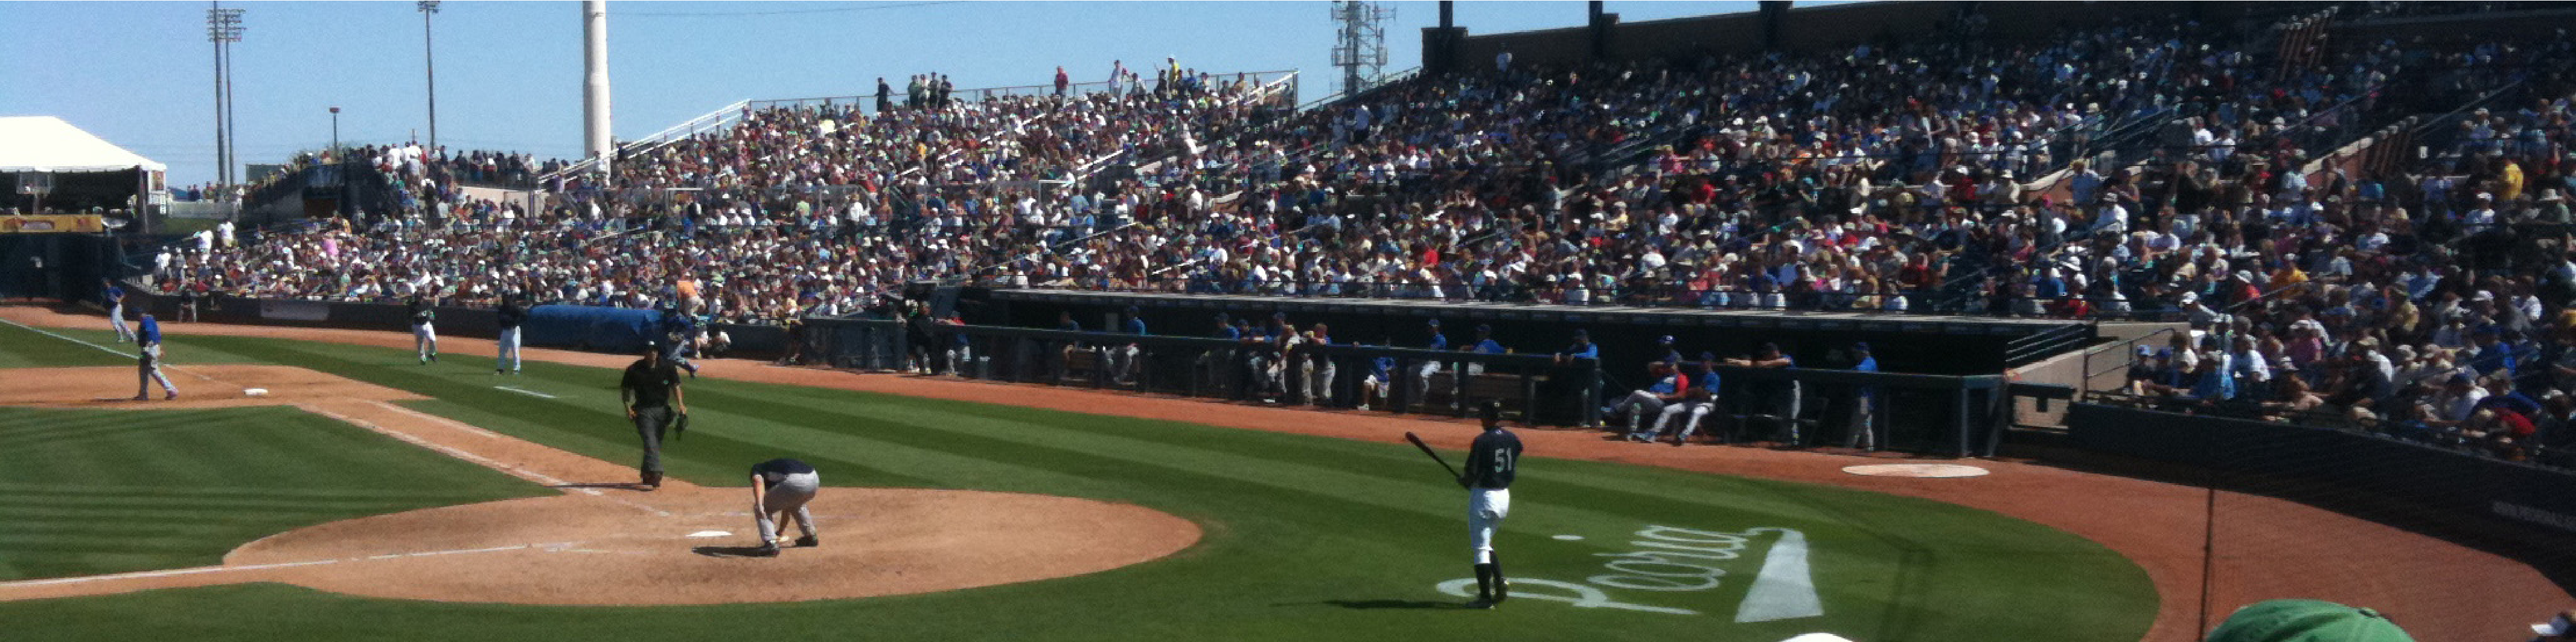
\includegraphics[width=\textwidth]{sampleteaser}
%   \caption{Seattle Mariners at Spring Training, 2010.}
%   \Description{Enjoying the baseball game from the third-base
%   seats. Ichiro Suzuki preparing to bat.}
%   \label{fig:teaser}
% \end{teaserfigure}

%%
%% This command processes the author and affiliation and title
%% information and builds the first part of the formatted document.
\maketitle

\section{Introdução}

O PAR Digital é uma ferramenta tecnológica desenvolvida com base em anos de estudo
e pesquisa pela Faculdade de Educação da Universidade Federal de Minas Gerais, PAR
significa Planejar, Aplicar, Rever, ações necessárias para que o ensino seja eficaz
para os alunos com deficiência.

\section{Objetivo}
O objetivo do PAR Digital é proporcionar uma ferramenta acessível e intuitiva
que facilite o preenchimento e a gestão do Plano Educacional Individualizado (PEI),
essencial para o desenvolvimento educacional dos alunos com deficiência. Desenvolvido
 a partir de princípios do Desenho Universal de Aprendizagem (DUA) e de uma parceria
 com o Atendimento Educacional Especializado (AEE), o sistema visa integrar-se de
 maneira eficiente na rotina diária dos educadores, promovendo um ensino inclusivo
 e personalizado.
% \url{https://www.acm.org/publications/proceedings-template}.

\section{Arquitetura}

A estrutura do projeto é organizada de maneira a facilitar 
a manutenção e a expansão do mesmo.

As principais tecnologias utilizadas no projeto incluem React.js, uma biblioteca
JavaScript para construção de interfaces de usuário, escolhida por sua eficiência
na criação de componentes reutilizáveis e desempenho otimizado. O TypeScript é
usado para adicionar tipagem estática ao código JavaScript, aumentando a robustez
e facilitando a manutenção. O Redux é empregado para o gerenciamento de estado da
aplicação, ideal para aplicações de médio e grande porte que necessitam de um
controle mais sofisticado do estado. A biblioteca Material-UI é utilizada para
implementar o design system do Google Material Design, enquanto o Axios serve
como cliente HTTP para realizar requisições a APIs. Ferramentas como Jest e
React Testing Library são utilizadas para testes automatizados, garantindo a
qualidade e a funcionalidade do código.

O fluxo de dados na aplicação é gerenciado pelo Redux, que centraliza o estado da
aplicação em um único store. As ações são despachadas a partir dos componentes,
que são tratadas pelos `reducers` para atualizar o estado global. Essa abordagem
facilita a depuração e o desenvolvimento de novas funcionalidades, uma vez que o
estado da aplicação se torna previsível e controlado.

A estilização da aplicação é feita utilizando CSS-in-JS com a biblioteca Material-UI,
 permitindo uma aplicação consistente do design system através dos componentes.
 A utilização de temas facilita a customização e a manutenção do estilo visual da
 aplicação.

Para a integração e entrega contínua (CI/CD), o projeto utiliza
o GitHub Actions, configurado para executar testes automatizados e builds a cada
commit, garantindo que a aplicação se mantenha estável e pronta para deployment.
O deploy é realizado em um servidor localizado na UFMG, permitindo uma escalabilidade
 fácil e eficiente.


% {\bfseries Your document will be returned to you for revision if
%   modifications are discovered.}

\section{Funcionalidades}

O projeto oferece diversas funcionalidades voltadas para o suporte
educacional de estudantes com necessidades especiais. A seguir, são
descritas as principais funcionalidades do sistema, cada uma desempenhando
 um papel crucial na promoção de um ambiente inclusivo e eficaz para o
 aprendizado

\subsection{CRUD de Usuários}
No sistema, os {\bfseries administradores} são responsáveis por gerenciar as
escolas, visualizando relatórios e detalhes como professores e
estratégias.
% \begin{verbatim}
%   \begin{teaserfigure}
%     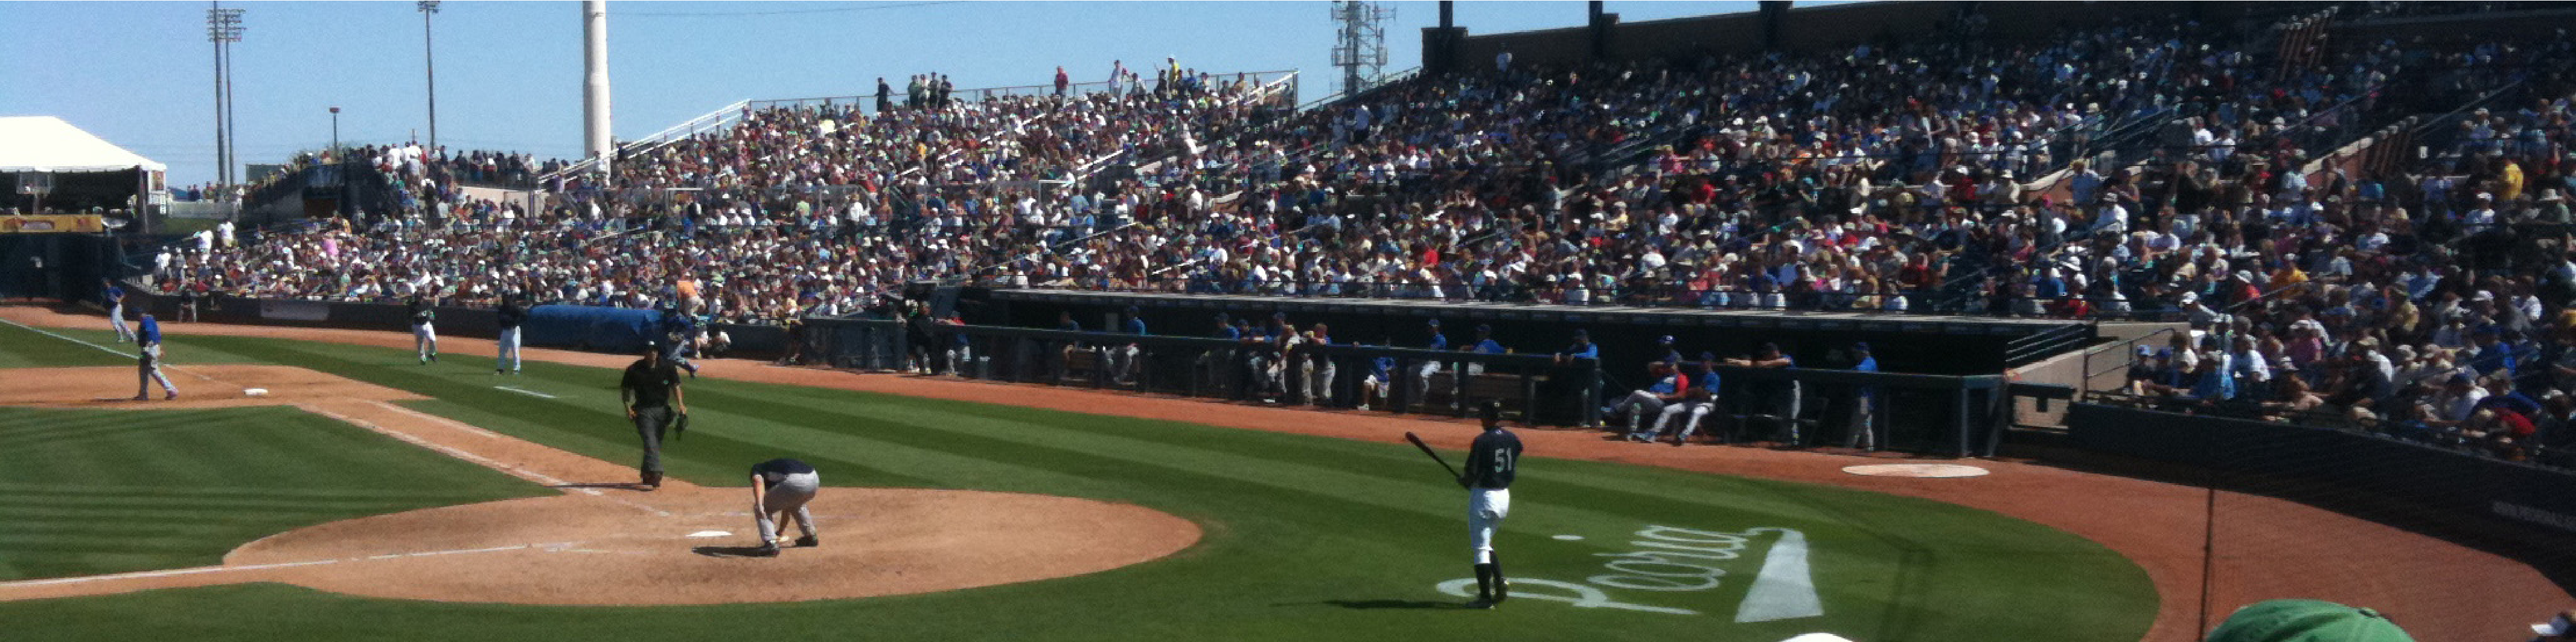
\includegraphics[width=\textwidth]{sampleteaser}
%     \caption{figure caption}
%     \Description{figure description}
%   \end{teaserfigure}
% \end{verbatim}
% \begin{figure}[h]
%   \centering
%   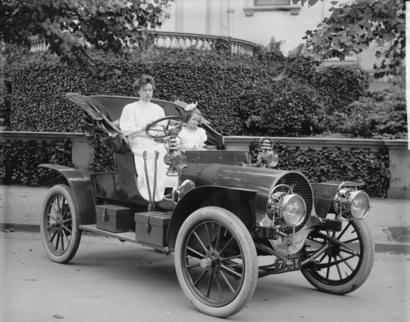
\includegraphics[width=\linewidth]{sample-franklin}
%   \caption{DANIELE}
%   \Description{tENTANDO COLOCAR UMA IMAGEM AQUI.}
% \end{figure}


As {\bfseries escolas}  criam professores, responsáveis e
desenvolvem o PEI, além de visualizar estratégias e dados dos alunos
e professores.

Os {\bfseries coordenadores}  acompanham o progresso dos alunos
e estratégias, visualizando o andamento dos alunos.

Os {\bfseries professores
regulares}  são os usuários chave, criando e aplicando estratégias, e
adicionando relatórios de progresso.

Os {\bfseries professores AEE}  auxiliam
os regulares, visualizando estratégias do PEI e relatórios, e
participando de fóruns.

Os {\bfseries responsáveis}  adicionam documentos
necessários e acompanham o desenvolvimento dos alunos, visualizando
seus dados e relatórios parciais.


\subsection{Criação do PEI}
A funcionalidade de criação do Plano Educacional Individualizado
(PEI) é uma das mais importantes, permitindo que educadores e 
coordenadores elaborem planos personalizados para atender às 
necessidades específicas de cada aluno.


\subsection{Estratégias do PEI}
Dentro do PEI, os educadores podem definir e documentar diversas 
estratégias pedagógicas adaptadas às necessidades do aluno. Essas 
estratégias são orientações práticas que guiam os professores na 
implementação do plano e ajudam a monitorar o progresso do aluno.

\subsection{Relatório sobre Estratégias}
A funcionalidade de relatórios permite que educadores e coordenadores 
acompanhem o andamento das estratégias definidas no PEI. 
Esses relatórios são fundamentais para avaliar o progresso do aluno, 
identificar áreas que necessitam de ajustes e garantir que as 
estratégias estão sendo eficazmente implementadas.

\subsection{Fórum de Acompanhamento do Aluno}
O fórum de acompanhamento do aluno é uma plataforma colaborativa onde 
professores, coordenadores e outros profissionais podem discutir o 
progresso do aluno, compartilhar insights e propor ajustes no PEI. 
Este fórum promove uma abordagem colaborativa e integrada ao 
acompanhamento educacional.

\subsection{Reutilização de Estratégias}
O sistema possui um banco de estratégias pedagógicas que podem ser 
reutilizadas. Educadores podem consultar esse banco para encontrar 
estratégias que já foram aplicadas com sucesso em situações similares
, facilitando a implementação de práticas comprovadamente eficazes.

\subsection{Compartilhamento de Recursos}
Uma funcionalidade vital do PAR Digital é o compartilhamento de 
recursos, especialmente Tecnologias Assistivas. Esse recurso 
permite que professores e coordenadores acessem ferramentas e 
materiais que podem ser utilizados para apoiar o aprendizado 
dos alunos com necessidades especiais.

\subsection{Perfil do Aluno}
O sistema mantém um perfil detalhado do aluno, que inclui informações
 educacionais e fundamentais. Esse perfil permite que educadores e 
 coordenadores tenham uma visão abrangente das necessidades, 
 capacidades e progressos do aluno, facilitando a personalização 
 do ensino e a monitorização do desenvolvimento educacional.



\section{Licença}
Software acadêmico, licença de tecnologias livres que está
 sendo utilizado de forma de cunho social?


\section{Perspectivas}

\subsection{Perspectiva Acadêmica}
O PAR Digital representa uma inovação significativa no campo 
da educação inclusiva, oferecendo uma ferramenta tecnológica 
poderosa para a gestão eficiente de Plano Educacional 
Individualizado (PEI). Academicamente, essa ferramenta pode 
servir como um catalisador para a pesquisa e o 
desenvolvimento contínuo de estratégias pedagógicas 
adaptativas. 

O acesso a dados detalhados sobre o progresso dos alunos, 
bem como o compartilhamento de estratégias bem-sucedidas 
entre os educadores, pode promover a produção de conhecimento
 acadêmico relevante na área da educação inclusiva. 

Além disso, o projeto pode facilitar estudos longitudinais 
sobre o impacto de intervenções específicas no 
desenvolvimento educacional de alunos com deficiência, 
fornecendo insights valiosos para a comunidade acadêmica.

\subsection{Perspectiva Social}
Socialmente, o PAR Digital tem o potencial de promover a 
inclusão e a igualdade de oportunidades na educação. Ao 
oferecer uma plataforma acessível e intuitiva para a 
gestão de PEIs, o sistema capacita os educadores a 
oferecer um suporte mais eficaz aos alunos com deficiência, 
adaptando seus métodos de ensino às necessidades 
individuais de cada estudante. Isso não apenas melhora 
a experiência educacional desses alunos, mas também 
fortalece a coesão social ao reconhecer e valorizar a 
diversidade no ambiente escolar.

Além disso, ao envolver os pais e responsáveis no processo 
educacional por meio do acompanhamento do progresso dos 
alunos, o software promove uma parceria colaborativa entre 
escola e comunidade, fortalecendo os laços sociais e a 
confiança na instituição educacional.

\section{Appendices}

If your work needs an appendix, add it before the \linebreak
``\verb|\end{document}|'' command at the conclusion of your source
document.

Start the appendix with the ``\verb|appendix|'' command:
\begin{verbatim}
  \appendix
\end{verbatim}
and note that in the appendix, sections are lettered, not
numbered. This document has two appendices, demonstrating the section
and subsection identification method.


%%
%% The acknowledgments section is defined using the "acks" environment
%% (and NOT an unnumbered section). This ensures the proper
%% identification of the section in the article metadata, and the
%% consistent spelling of the heading.
\begin{acks}
To Robert, for the bagels and explaining CMYK and color spaces.
\end{acks}

%%
%% The next two lines define the bibliography style to be used, and
%% the bibliography file.
\bibliographystyle{ACM-Reference-Format}
\bibliography{sample-base}

%%
%% If your work has an appendix, this is the place to put it.
\appendix

\section{Research Methods}

\subsection{Part One}

Lorem ipsum dolor sit amet, consectetur adipiscing elit. Morbi
malesuada, quam in pulvinar varius, metus nunc fermentum urna, id
sollicitudin purus odio sit amet enim. Aliquam ullamcorper eu ipsum
vel mollis. Curabitur quis dictum nisl. Phasellus vel semper risus, et
lacinia dolor. Integer ultricies commodo sem nec semper.

\subsection{Part Two}

Etiam commodo feugiat nisl pulvinar pellentesque. Etiam auctor sodales
ligula, non varius nibh pulvinar semper. Suspendisse nec lectus non
ipsum convallis congue hendrerit vitae sapien. Donec at laoreet
eros. Vivamus non purus placerat, scelerisque diam eu, cursus
ante. Etiam aliquam tortor auctor efficitur mattis.

\section{Online Resources}

Nam id fermentum dui. Suspendisse sagittis tortor a nulla mollis, in
pulvinar ex pretium. Sed interdum orci quis metus euismod, et sagittis
enim maximus. Vestibulum gravida massa ut felis suscipit
congue. Quisque mattis elit a risus ultrices commodo venenatis eget
dui. Etiam sagittis eleifend elementum.

Nam interdum magna at lectus dignissim, ac dignissim lorem
rhoncus. Maecenas eu arcu ac neque placerat aliquam. Nunc pulvinar
massa et mattis lacinia.

\end{document}
\endinput
%%
%% End of file `sample-sigconf.tex'.
